\documentclass{beamer}
\usepackage{graphicx}
\graphicspath{{images/}}
\usepackage{pgf}
\usepackage{xfrac}
\newcommand\inputpgf[2]{{
\let\pgfimageWithoutPath\pgfimage
\renewcommand{\pgfimage}[2][]{\pgfimageWithoutPath[##1]{#1/##2}}
\input{#1/#2}
}}



\usepackage{physics}

\usepackage{mathtools}  
\mathtoolsset{showonlyrefs} 

\mode<presentation>{}

\usefonttheme{serif}

%% preamble
\title{Quantum particle on a circle}
%\subtitle{The subtitle}
\author{Riccardo Antonelli}
\begin{document}

\begin{frame}
    \maketitle
\end{frame}

\begin{frame}{Divergent oscillations}
\begin{equation*}
    \mathcal{A} = \sum_{\phi(t)} e^{iF[\phi(t)]}
    \label{}
\end{equation*}

Quantum observables are oscillatory sums\footnote{politically correct language for ``divergent''}, need \textbf{regularization}.

\end{frame}

\newcommand{\imt}{\eta}

\begin{frame}{Wick rotation}
    Standard answer: tilt head $\pi/2$.

    \begin{equation}
        t = i\imt
        \label{}
    \end{equation}

    \begin{equation}
        F[\phi(i\imt)] = i \mathcal{F}[\varphi(\imt)]
        \label{}
    \end{equation}

    \begin{equation}
        \mathcal{A}(it) = \sum_{\varphi(\imt)} e^{-\mathcal{F}[\varphi(i\imt)]}
        \label{}
    \end{equation}

    Now they converge. Then hopefully get back to real axis through analytic continuation.
\end{frame}

\begin{frame}{QM on circles}
    Place free quantum particle on a circle.

    \begin{align}
        x \sim x + 1\,, && \psi(x+1,t) = \psi(x,t)\\
        i \pdv{t} \psi(x,t) = - {\Delta \over 2} \psi(x,t) && \partial_x \psi(x+1,t) = \partial_x \psi(x,t)
        \label{}
    \end{align}
    
    Initial condition is a position (generalized) eigenstate

    \begin{equation}
        \psi(x,0) = \delta(x)
        \label{}
    \end{equation}

    $\psi(x,t)$ is the \textbf{propagator} or \textbf{fundamental solution}.

\end{frame}

\newcommand{\sumZ}{\sum_{n=-\infty}^\infty}

\begin{frame}{Unwrapping the circle}
    On $\mathbb{R}$, the propagator is innocuous enough:

    \begin{equation}
        G_\mathbb{R}(x,t) = {1 \over \sqrt{ 2\pi i t }} \exp(ix^2 \over 2t)
        \label{}
    \end{equation}

    But $\mathbb{S}^1 = \mathbb{R} / \mathbb{Z}$, therefore

    \begin{equation}
        G(x,t) = \sumZ G_\mathbb{R}(x+n,t) 
    \end{equation}
    \begin{equation}
        = \exp(ix^2 \over 2t) {1 \over \sqrt{2\pi i t}} \sumZ \exp( {in^2 \over 2t} + {ixn \over t} )
    \end{equation}

    Simply a \textbf{method of images}!
\end{frame}

\begin{frame}{Unwrapping the circle II}
    \scalebox{0.8}{    \input{images/wrapping.pdf_tex}}
\end{frame}


\begin{frame}{A pleasant surprise}
    \begin{equation}
   G(x,t) = \exp(ix^2 \over 2t) {1 \over \sqrt{2\pi i t}} \sumZ \exp( {in^2 \over 2t} + {ixn \over t} ) 
   \end{equation}

   Change variables $\tau := 2\pi t$, $z := x$, and use Poisson resummation:

   \begin{equation}
       G(z,\tau) = \sumZ \exp(\pi i n^2 \tau + 2 \pi i n z)
       \label{}
   \end{equation}

   It's the Jacobi $\vartheta$ function!
\end{frame}

\newcommand{\T}{\vartheta}

\begin{frame}{A less pleasant surprise}

    $\T(z,\tau)$ is defined and holomorphic for $\Im \tau > 0$, but \textbf{time is real}!
    
    \vfill

    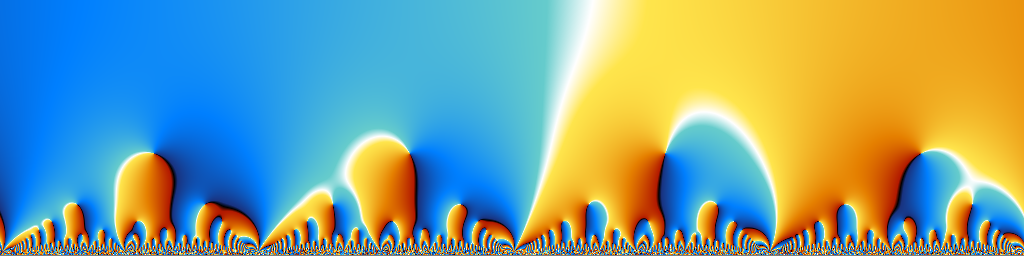
\includegraphics[width=\textwidth]{images/plots/theta_new}

    \vfill

    Is there any hope of making sense of $\T(z,\tau)$ for real periods?

\end{frame}

\begin{frame}
    \begin{center}\Large Set $z=0$ for now.
    \vfill
    (physically: final point $=$ starting point)
\end{center}
\end{frame}

\begin{frame}{The propagator exists}
    $\T(z,\tau)$ for real $\tau$ \textbf{is} well defined, but as a tempered distribution. Indeed, for Schwartz $\phi(\tau)$:

    \begin{equation}
        \int d\tau \phi(\tau) \T(0,\tau) = \sumZ \int d\tau \phi(\tau) e^{i\pi n^2 \tau} = \sumZ \hat\phi(-\pi n^2) \in \mathbb{C}
        \label{}
    \end{equation}

    \vfill

    However, \emph{what} distribution is it? It is neither induced by an $L^1_{loc}$ function, nor does it have any part with single point support ($\delta$-like).
\end{frame}

\begin{frame}{The even modular group}
    $\T(0,\tau)$ has remarkable transformation properties under modular transformations.

\begin{equation}
    \T(0,\tau + 2) = \T(0,\tau)\,,\quad \T\left(0,-\frac{1}{\tau}\right) = \sqrt{-i\tau} \T(0,\tau)
    \label{}
\end{equation}

All rational times $p/q$ can be mapped back to either $1$ or $0$ depending on the parity of $pq$.

\begin{center}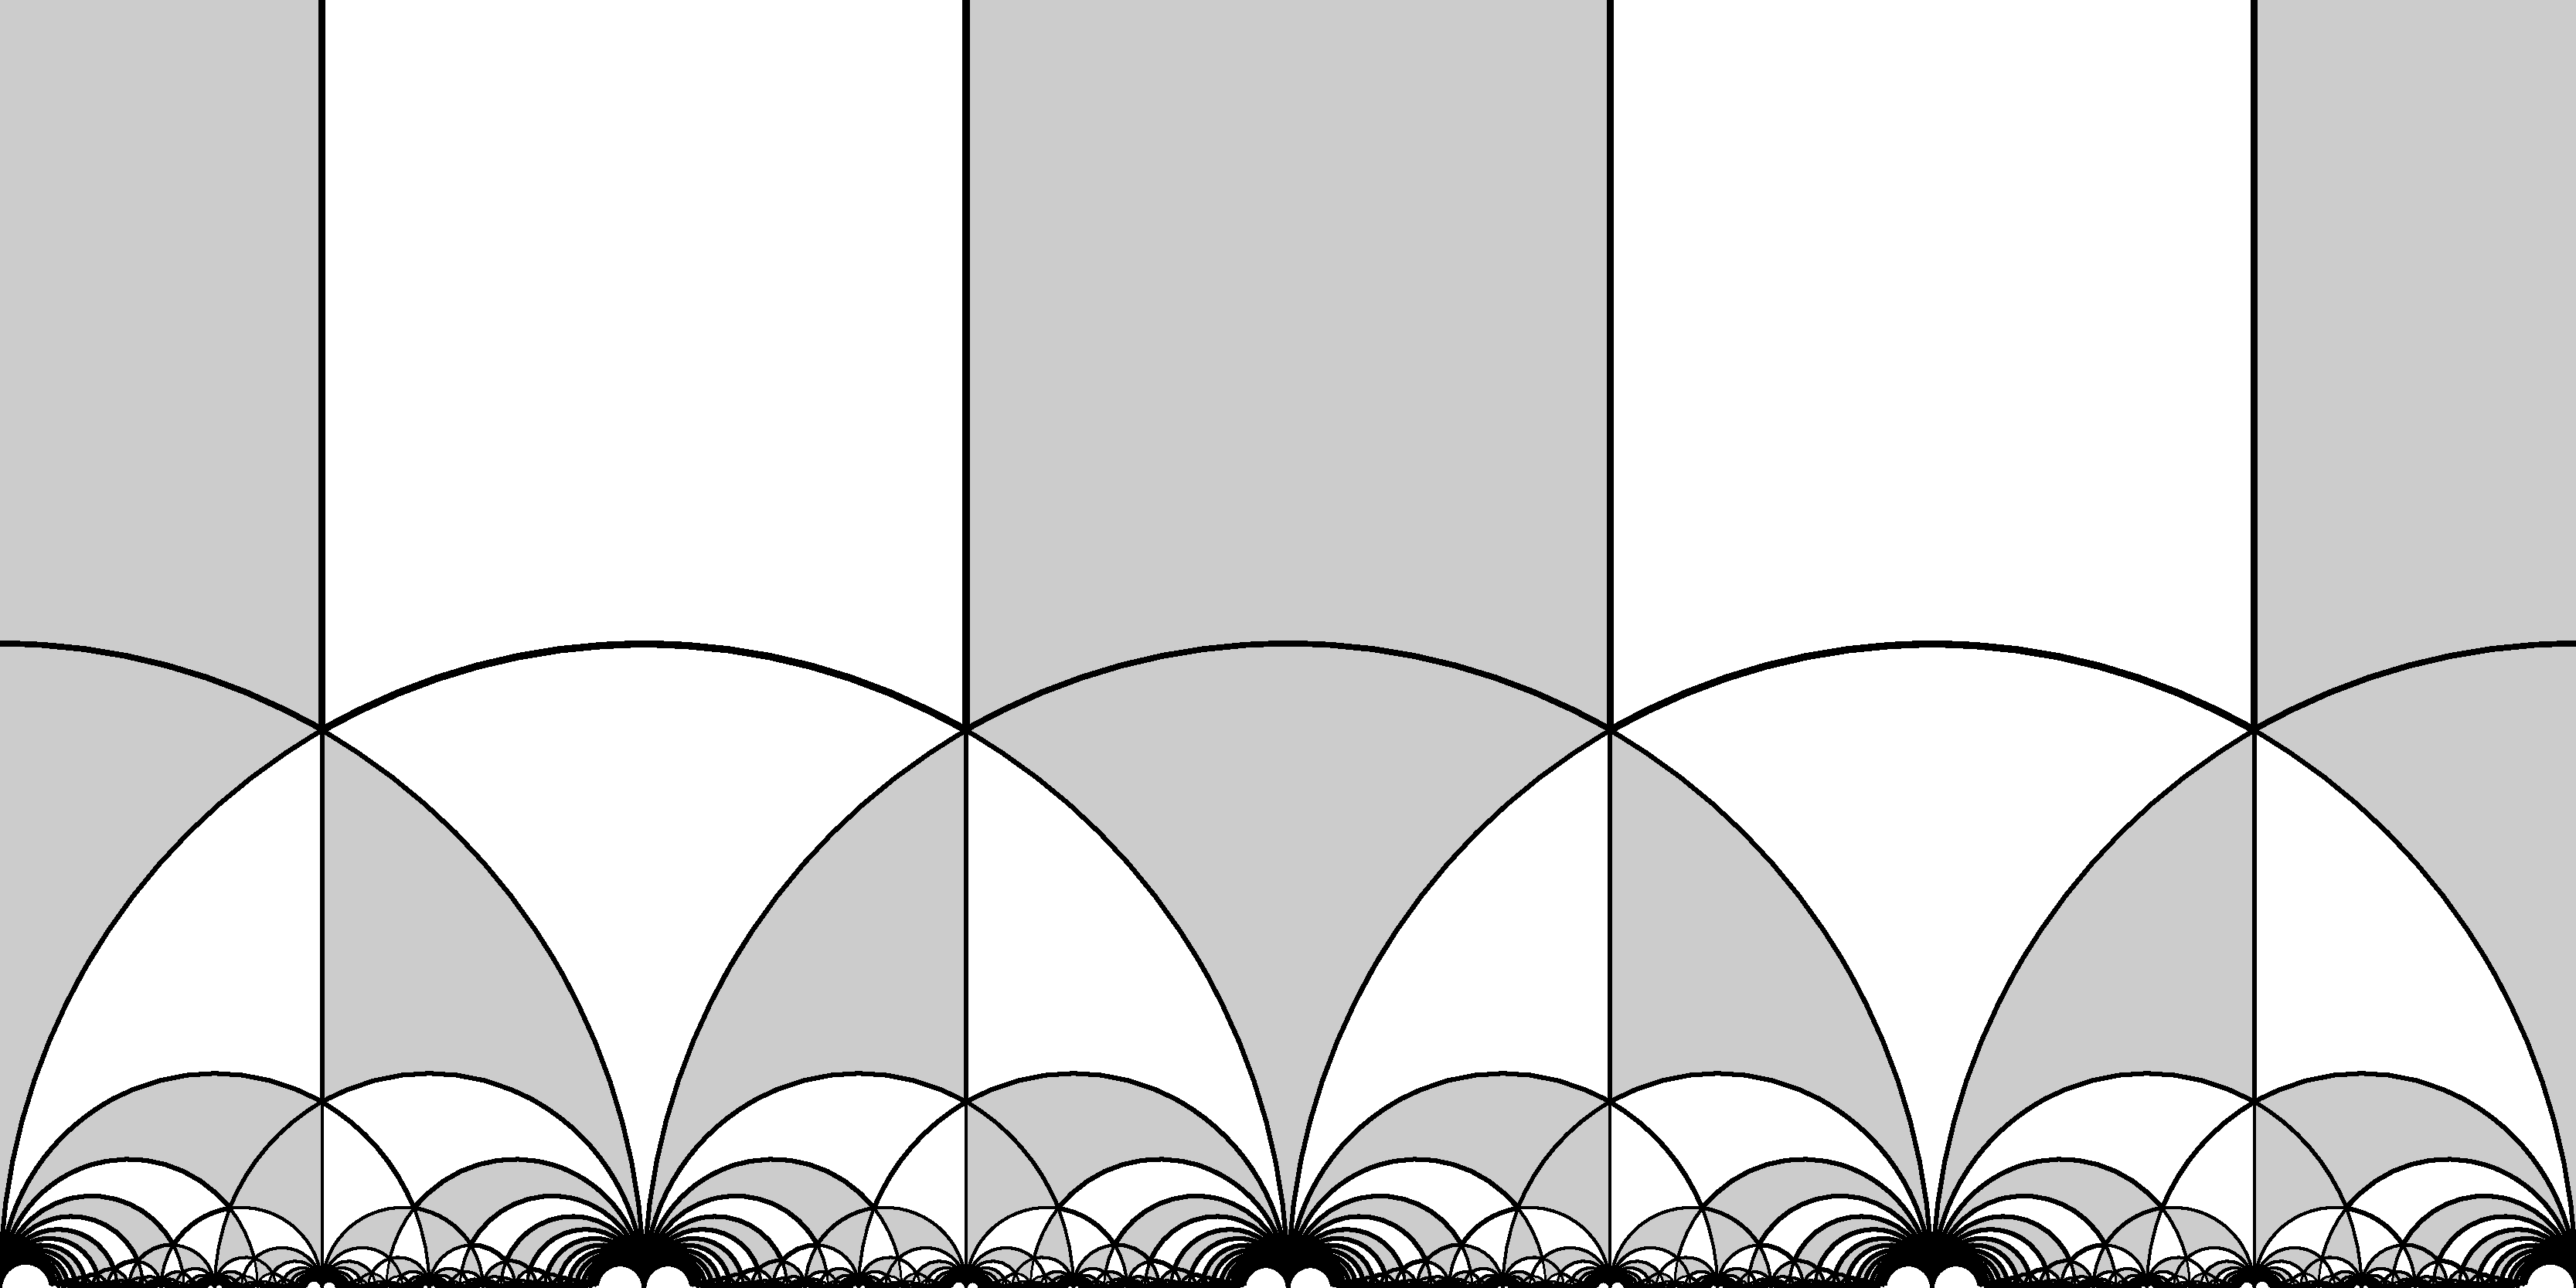
\includegraphics[width=0.8\textwidth]{modulargroup}\end{center}

\end{frame}


\begin{frame}{Self-similarity}
    Self-similar structure:

    \begin{center}
        \Large The behaviour around $\tau = 0$ is repeated at all even rationals. The behaviour around $\tau=1$ is repeated at all odd rationals.
    \end{center}
\end{frame}

\begin{frame}{Even rationals}
        $\T(\tau)$ is ``asymptotic'' to $1/\sqrt{\tau}$ for $\tau \rightarrow 0$. Normal analytic methods however fail. We test with shrinking gaussian test functions:
\begin{equation}
    \left\langle g_\sigma(\tau), \T \right\rangle \sim \left\langle g_\sigma(\tau) , \tau^{-1/2} \right\rangle
    \label{}
\end{equation}

\vfill

        \[\int d\tau \, \vartheta(\tau) \frac{1}{\sigma\sqrt{2\pi}} e^{-\frac{\tau^2}{2\sigma^2}} = \sumZ \exp(-\pi^2 \sigma^2 n^4 / 2) \]
    
        \[\sim \frac{2^{1/4}}{\sqrt{\pi \sigma}} \int d\xi e^{-\xi^4} = \frac{2^{-3/4}}{\sqrt{\pi\sigma}} \Gamma\left(\frac{1}{4}\right) \]


        \[ \int d\tau \, \frac{1}{\sqrt \tau} \frac{1}{\sigma \sqrt{2\pi}} e^{-\frac{\tau^2}{2\sigma^2}}  = \frac{2^{-3/4}}{\sqrt{\pi \sigma}} \Gamma\left(\frac{1}{4}\right) \]


\end{frame}

\begin{frame}



\vfill

Modular symmetry $\Rightarrow$ there is a $(\Delta \tau)^{-1/2}$ singularity near all even $p/q$. In particular we find:

\begin{equation}
    \T(\tau) \sim \frac{1}{\sqrt{p - q\tau}}
    \label{}
\end{equation}

$\theta(\tau)$ has a \textbf{dense} set of singularities! They are rescaled by $1/\sqrt{q}$.



\end{frame}

\begin{frame}{Odd rationals}
    For $\tau \rightarrow 1$, $\T \rightarrow 0$, and all derivatives $\dv[k]{\tau} \T \rightarrow 0$, again as a distributional limit:

   
    \begin{equation}
        \left\langle g_\sigma(\tau-1), \dv[k]{\tau} \T \right\rangle \rightarrow 0\,,\quad \sigma \rightarrow 0\,,\; k = 0,1,2,\ldots
        \label{}
    \end{equation}

    \vfill

   
    \[ \propto \sumZ n^{2k} (-1)^n e^{-\pi^2 \sigma^2 n^4 / 2} = \frac{1}{2\pi i}\oint \frac{\pi}{\sin \pi z} z^{2k} \exp(-\pi^2\sigma^2 n^4) dz \]

    \begin{columns}
        \begin{column}{0.5\textwidth}
        \centering        \scalebox{0.8}{\input{images/contour.pdf_tex}}
        \end{column}
        \begin{column}{0.5\textwidth}

        Send $\sigma \rightarrow 0$, but keep $l \sqrt{\sigma}$ constant.
        \end{column}
    \end{columns}

\end{frame}

\begin{frame}

    Modular symmetry $\Rightarrow$ there is a ``flat point'' at all odd $p/q$. $\T(\tau)$ has a \textbf{dense} set of zeroes!


\end{frame}

\begin{frame}{Plot of $\T(\tau)$?}
    Plotting $\T(\tau)$ doesn't really work\ldots
    
    \begin{centering}
        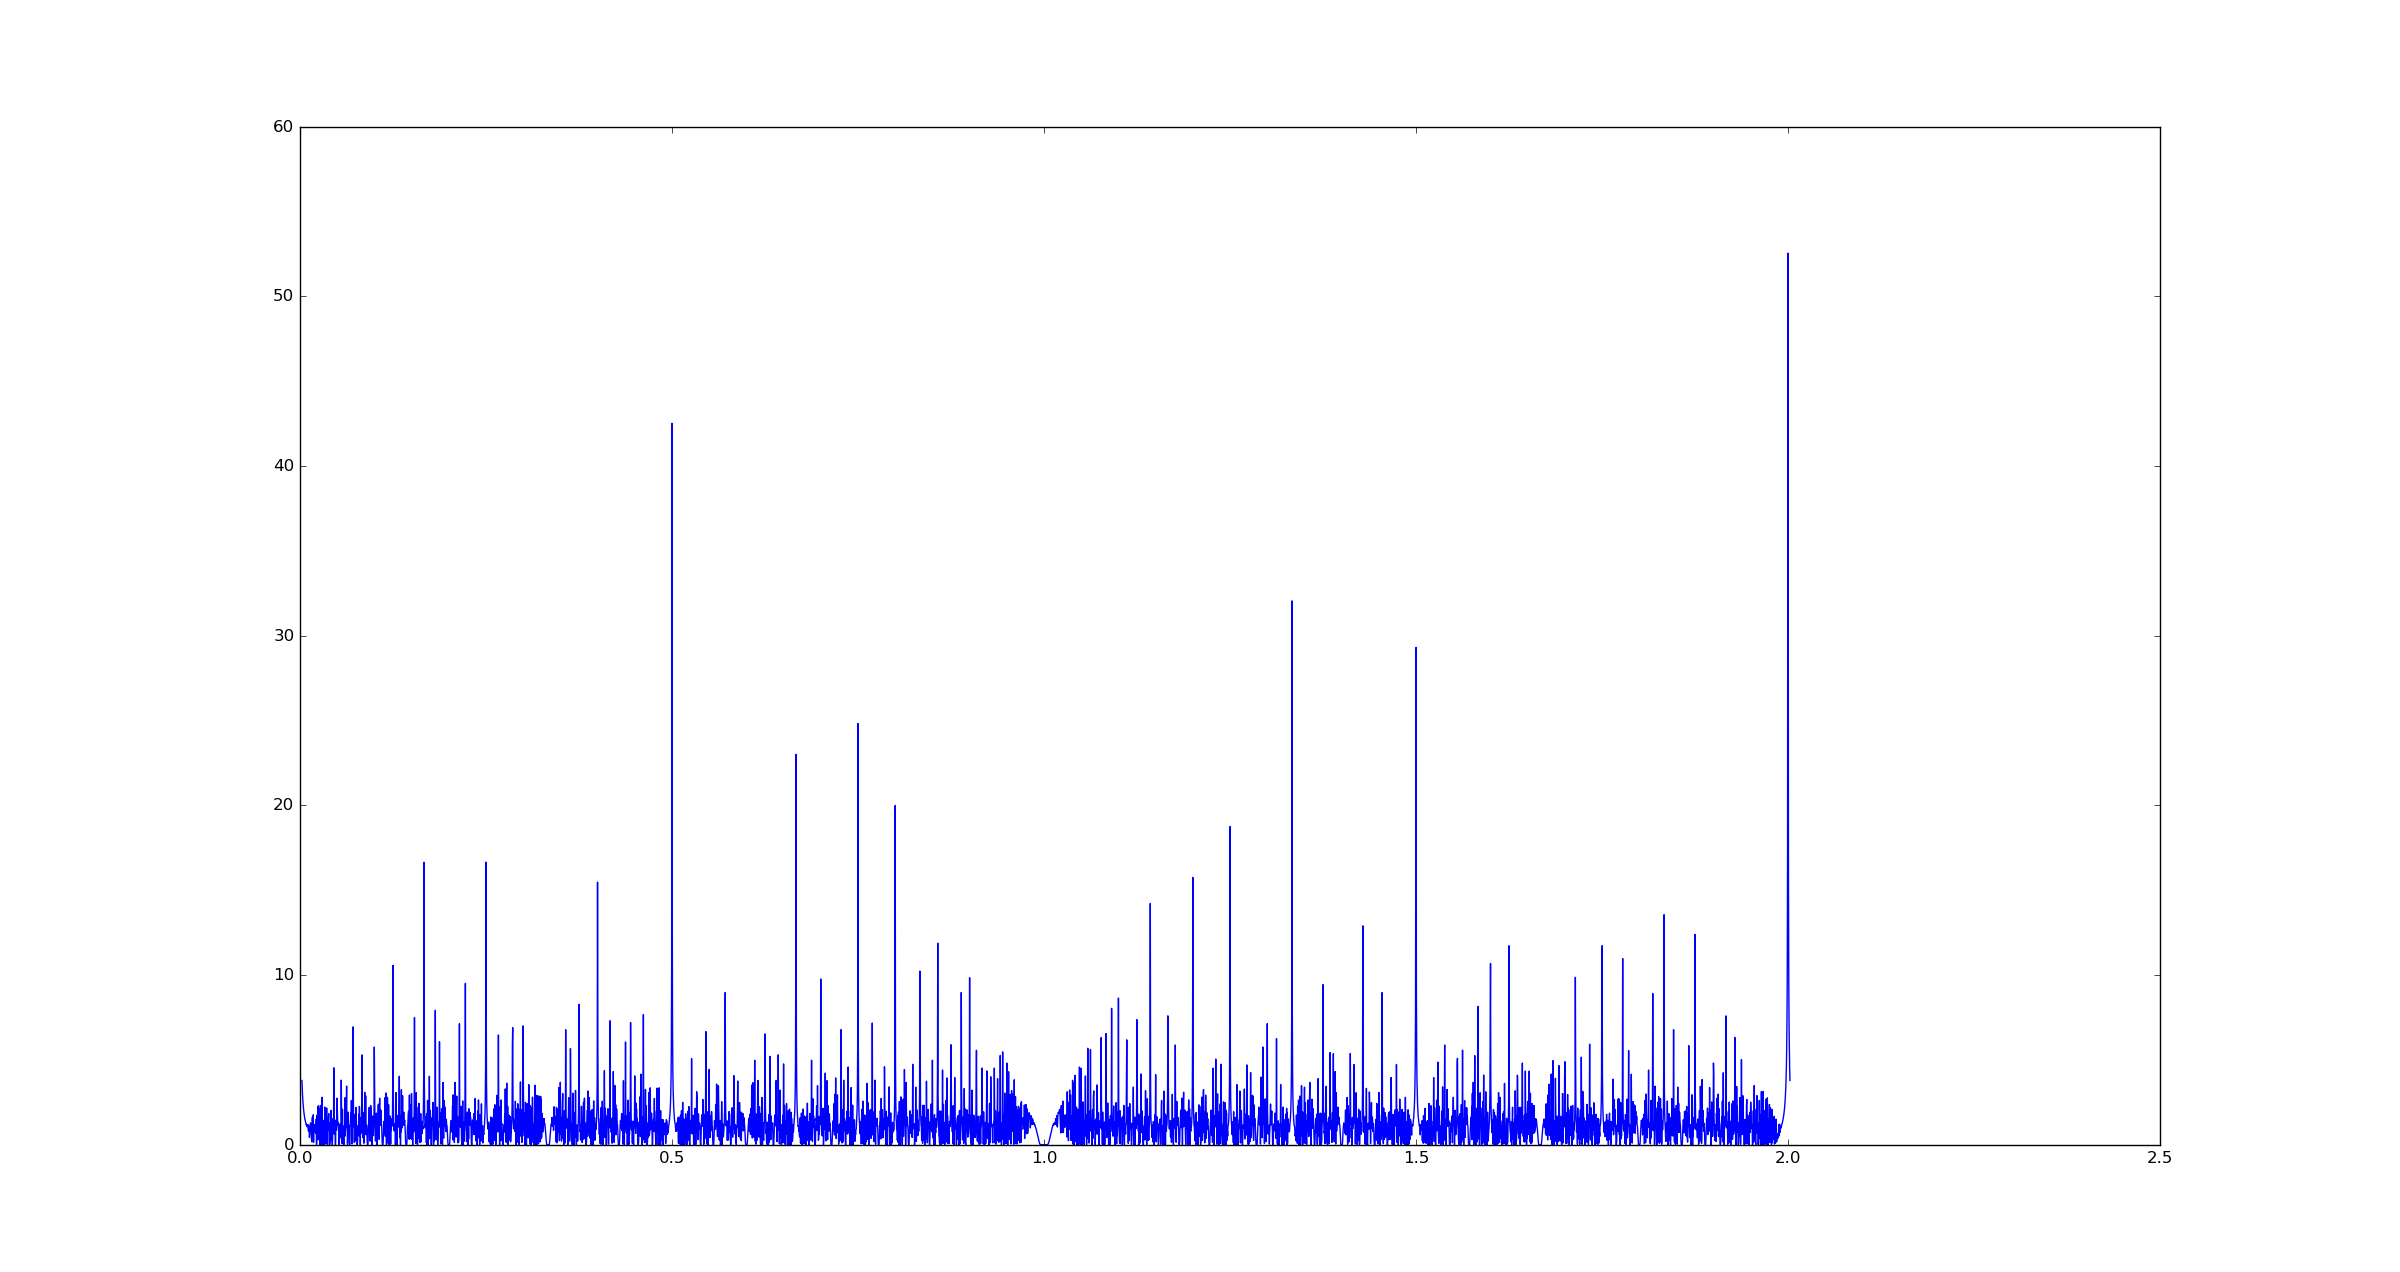
\includegraphics[width=1.2\textwidth]{figure_1}
    \end{centering}

\end{frame}


\begin{frame}{Plot $B(\tau) = \int d\tau \T(\tau)$}
    Plot distributional antiderivative $B(\tau) := \sumZ \frac{2}{i\pi} \frac{e^{i\pi n^2 \tau}}{n^2}$

    \scalebox{0.8}{\inputpgf{images}{batman.pgf}}
\end{frame}


\begin{frame}
    Fix $\tau = p/q$, study $z$ dependence.

    \begin{equation}
        \vartheta\left(z,\frac{p}{q}\right) = \sumZ e^{\pi i n^2 \frac{p}{q} + 2\pi i n z}
        \label{}
    \end{equation}

    Trick: $n = aq + b$, $a \in \mathbb{Z}$, $b = 0,\ldots,q-1$

\begin{equation}
    \vartheta\left(z,\frac{p}{q}\right) = \frac{1}{\sqrt q} \sum_{c=0}^{q-1} \phi_{p,q,c} \, \delta\left(z - \frac{c+\Delta}{q}\right)
    \label{}
\end{equation}


The propagator is a ``\textbf{fractional comb}'' of $q$ equally-spaced $\delta$-functions.

\vfill

{\small $\Delta := (-1)^{pq}/2$}

\end{frame}

\begin{frame}

Phases $\phi_{p,q,c}$ are quadratic Gauss sums!

\begin{equation}
    \phi_{p,q,c} = \sqrt{q} \sum_{b=0}^{q-1} (e^{i\pi/q})^{pb^2 + 2bc + 2\Delta b}
    \label{}
\end{equation}

No general closed form.

\end{frame}

\begin{frame}{Back to physics}
    Periodicity $\vartheta(z,\tau + 2) = \vartheta(z,\tau)$ is expected physically: \textbf{quantum revival}.

   \vfill

    If $E_n = m_n E$, $m_n \in \mathbb{Z}$, then state is periodic in time:

    \begin{equation}\Psi(t + 2\pi/E) = \Psi(t)\end{equation}

\end{frame}


\begin{frame}
    However at $\tau \in \mathbb{Q}$ initial state is ``cloned'' into $q$ reduced and shifted copies: \textbf{fractional revival}

    \begin{center} 
        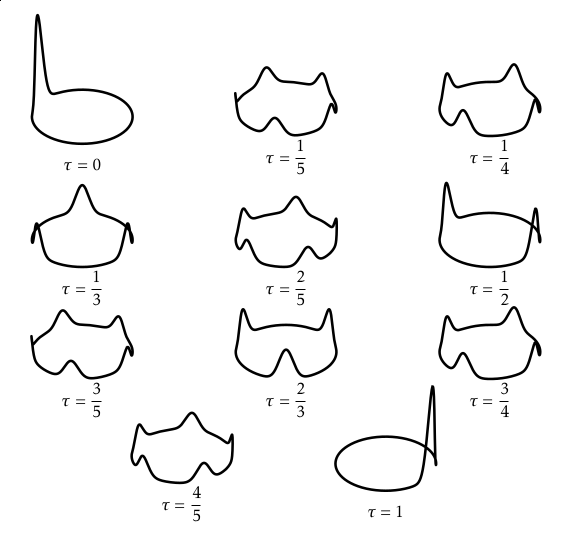
\includegraphics[scale=0.4]{images/mergiata2}
    \end{center}
\end{frame}

\begin{frame}
    What is the physical origin of fractional revivals?

    \vfill

    Heuristic reasoning: apply saddle point to path integral:

    \begin{equation}
        \mathcal{A} = \int D\phi e^{iS[\phi_{cl}]} (1 + \text{oscillatory}\ldots)
        \label{}
    \end{equation}

    \vfill

    But if there are infinite $\phi_{cl}$, $\mathcal{A}$ would diverge\ldots

    \vfill
\end{frame}

\begin{frame}
    Reconvergence of classical solutions, a \textbf{caustic}, generates a $\delta$-function singularity in an amplitude (simply resonance!). 
    
    \vfill

    When $2\pi t$ is rational, then an infinite number of classical solutions starting at $z=0$:

    \begin{equation}
        z_v(t) = vt\,;\quad v = 2\pi {n \over p}
        \label{}
    \end{equation}


    will reconverge at the $q$ points $0$, $1/q$, $2/q$, \ldots, $(q-1)/q$.
\end{frame}

\begin{frame}
\makebox[\textwidth][c]{
    \scalebox{0.8}{\inputpgf{images/}{butterfly.pgf}} }
\end{frame}

\end{document}
